\section{Background of air pollution}
\label{sec:background}

\BL{A}ir pollution is a mixture of particles and gases, often not visible to human
eyes. The visible forms are widely known, such as smoke, soot and mold.
According to Conselho Nacional do Meio Ambiente (CONAMA)
\cite{conama-air-pollution}, atmospheric pollution is 

\begin{quotation}
    ``... any form of matter or energy with intensity and in quantity,
    concentration, time or characteristics in disagreement with the
    established levels, and that make or may make the air: inappropriate,
    inconvenient, harmful to the environment or harmful to safety.''
\end{quotation}

Different anthropogenic process emit air pollutants, such as, for instance,
fossil fuels (motor traffic and domestic), agriculture, and industries.
Besides that, natural disaster are an important gas emitter, not controllable,
though. 

\subsection{Polluting gases}
\label{sec:polluting-gases}

The atmosphere of the Earth is a dynamic and complex system of natural gases,
which are necessary to life \cite{gases}. The planet has a defense mechanism
that absorbs part of them. However, high levels of gases concentration can cause several effects in the
living beings. Air pollutants are divided according to their origin \cite{who2006}: 

\begin{itemize}
    \item {\bf Primary:} those emitted into the atmosphere from a source; or
    \item {\bf Secondary:} those formed within the atmosphere through a
    chemical reaction.
\end{itemize}

Other important distinctions are related to their chemical class - organic or
inorganic, and related to their physical state - gaseous or particulate. The
selected pollutants are: 

\begin{itemize}
    \item \textbf{Carbon monoxide (CO):} CO results of incomplete combustion
    of matter with carbon and it does not present smell or color. Its
    concentration level is strongly related to car traffic, in addition to
    agricultural and forest fires. When breathed, it reduces the ability of
    oxygen transport by the hemoglobins.  

    \item \textbf{Ozônio (O$_3$):} It exists naturally in the atmosphere,
    where it has the function of absorbing ultraviolet radiation from the sun
    and of reducing its impact on the planet Earth surface. Nitrogen oxides and
    organic compounds, with oxygen and high temperatures form the ozone. However, in
    the troposphere, it is toxic and even explosive. Its
    effect on health can be drastic. 

    \item \textbf{Particulate matter (PM$_{10}$):} It is composed by particles
    of solid or liquid matter suspended in the air, with 10 micrometers of
    less. Combustion is one of the major human sources of particulate matter.
    Its effects include respiratory tract infections and damages to the
    environment. When the aerodynamic diameter is between 2.5 and 10
    micrometers, we call it PM$_10$, and it is the most common among the
    suspended particles measured.  

\end{itemize}

Other measured pollutants that we will not study by computacional and data
limitations are Sulfur Dioxide (SO$_2$), Nitrogen Oxides (NOx), and Hydrocarbons (HC).

\subsection{Urban air quality problems}

Air pollution episodes, such as, for example, the 1930 Meuse Valley in Belgium
\cite{nemery2001}, the 1952 Great Fog of London
\cite{polivka2018}, and the 2006 Southeast Asian Haze \cite{jones2006} raised
questions and concerns about high levels of pollutants in urban ambients,
which caused several deaths and hospitalizations. The rapidly expanding
populations and cities also increase the exposure to them.

In Brazil, in the last decade, more than 60,000 died on average per year due
to air pollution \cite{data-deaths-air-pollution}. Household air pollution
from solid fuels caused most of the cases, followed by ozone pollution, and
particulate matter pollution. 

\subsection{Air quality index}

The air quality index is a synthetic indicator what simplifies the divulgation
and the communication among population, private and public sectors, ONGs, etc.
Its divulgation is made through diary reports for each monitoring
station\footnote{\url{http://jeap.rio.rj.gov.br/je-metinfosmac/boletim}} as
shown in Figure \ref{fig:boletim}. 

The index considers the pollutants PM$_{10}$, PM$_{2.5}$, O$_3$,
CO, NO$_2$, and SO$_2$. For each one, The AQIr is calculated as follows,
\begin{equation}
    \label{eq:AQI}
    AQIr = I_{ini} + \frac{I_{fin} - I_{ini}}{C_{fin} - C_{ini}} \times (C - C_{ini}), 
\end{equation}
such that $I_{ini}$ ($I_{fin}$) is the value of the index that corresponds to
the initial (final) concentration of the range; $C_{ini}$ ($C_{fin}$) is the
initial (final) concentration of the range in which the measured concentration
is located, and $C$ is the concentration measured. The value informed is the
maximum $AQIr$ of the pollutants. 

After calculating the AIQ, we classify air quality at five levels: N1 (0-40),
N2 (41-80), N3 (81-120), N4 (121-200), and N5 ($>$ 200). For more details,
consult the technical guide from the Ministry of the Environment \cite{guia-tecnico-mma}. 

\begin{figure*}[!ht]  
    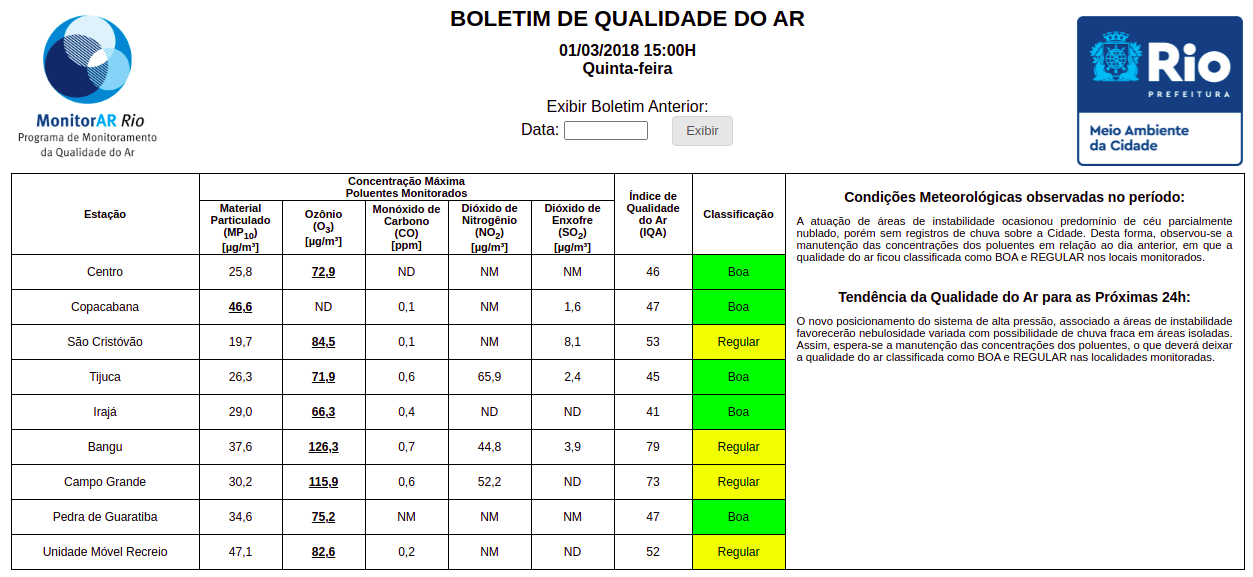
\includegraphics[width=\linewidth]{../images/boletim01-03-2018.png}
    \caption{Report from March 1$^{st}$, 2018.}
    \label{fig:boletim}
\end{figure*}



